\section{Ausrichten der Wände auf die Hauptachsen (Janneke)}

Bisher haben wir die Translation der Karte um andere Bewegungen des Roboters auszugleichen noch gar nicht beachtet. Hierfür können X- und Y-Histogramme verwendet werden. Um ein X- bzw. Y-Histogramm zu erstellen muss allerdings der Scan hauptachsenaligned sein. D.h. das die Wände bzw. geraden Linien im Scan auf der X- bzw Y-Achse liegen muss.

Dies könnte man nur für die Erstellung der Histogramme in jedem Schritt für jeden Scan einzeln machen, wir haben uns jedoch dafür entschieden unseren initialen Scan so auszurichten da dann jeder weitere Scan durch die Rotationskorrektur auf den ersten Scan ausgerichtet wird und damit automatisch auch auf die Hauptachsen ausgerichtet wird.

Also suchen wir das Maximum im Winkelhistogramm des ersten Scans welches der prominentesten Wand entsprechen würde. Dann rotieren wir den Scan so, dass der berechnete Winkel auf die Null im Histogramm verschoben wird. Diese Rotation setzen wir dann als initialen Rotationsoffset. Der rotierte Scan wird dann in die Karte eingezeichnet, sodass unsere resultierende Karte auch direkt Hauptachsenaligned ist.

\begin{figure}
	\centering
	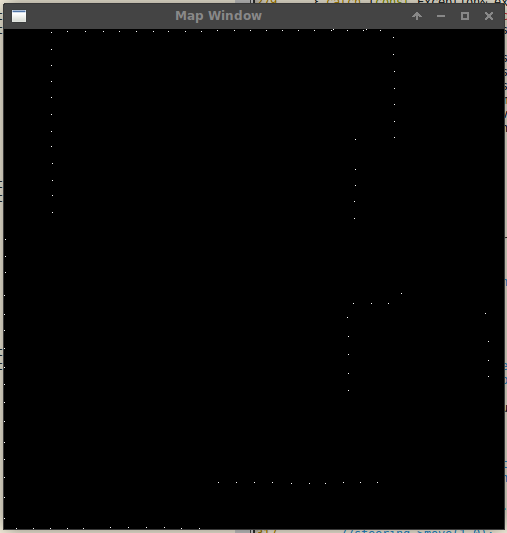
\includegraphics[width=11cm]{hauptachsenalignedMap}
	\caption{Auf die Hauptachsen ausgerichtete Karte}
	\label{fig:Hauptachsenaligned}
\end{figure}

Abbildung~\ref{fig:Hauptachsenaligned} zeigt die Karte in die der initiale auf die Hautachsen ausgerichteten Scan eingezeichnet ist.